\chapter{Extended Source Detection above 50 GeV: The 2FHL Catalog}
\label{chap:2FHL}

Application of addSrcs searching for extended (and really point too) sources in the sky. 2FHL results on all Galactic sources. Index histograms for entire \twofhl population showing harder index for Galactic sources.

We don't just detect extended though! The pipeline was built to try extended and if that's not likely, revert to point source. Simple check with Alberto's pipeline to show we didn't detect any glaring discrepancies. Quick check of Alberto's results for clusters of point source at \blat.

How much of the 2FHL paper can I put in as is, how much can I take with modifications?

Below is if I just took the sections describing extend sources. 

Something about connecting to \tev{}
\section{\label{sec:3FGL_ES}Extended Sources Previously Detected by the LAT}
We explicitly modeled sources as spatially extended when a previous, dedicated, analysis found the source to be resolved by the LAT.
The 25 extended sources reported in 3FGL were included in our model using the spatial templates derived in the individual source studies \citep[see references in ][]{3FGL}. Refitting the positions and extensions of the 3FGL extended sources in this energy range is beyond the scope of this work.

Of the 25 3FGL extended sources, 19 are significantly detected here above the detection threshold (${\rm TS}\geq25$). Only 6 sources are not detected and, since all have  ${\rm TS<10}$, are removed from the sky model (see \S\ref{sec:ESresults} for details).

One extended LAT source has had a dedicated analysis published since the release of the 3FGL catalog. \cite{HESSLATW41} reported joint H.E.S.S. and LAT observations of the very high energy (VHE) source HESS~J1834-087. This source is coincident with supernova remnant (SNR) W41 and was detected  as spatially extended in a wide energy range spanning 1.8\,GeV to 30\,TeV. In this paper, we employ the spatial model for the GeV emission determined in \cite{HESSLATW41}, leading to a significant detection of this source.


%%%%%%%%%%%%%%%%%%%%%%%%%%%%%%%%%%%%%%%%%%%%%%%%%%%%%%%%%%%%%%%%
%
%         Extended Sources not in 3FGL
%
%%%%%%%%%%%%%%%%%%%%%%%%%%%%%%%%%%%%%%%%%%%%%%%%%%%%%%%%%%%%%%%%
\section{\label{sec:newES}Newly Detected Extended Sources} %\jamie{should this be changed to something like ``Newly Detected Extended Sources" since W41 is now included in the previous section and is not a 3FGL source?}

In addition to modeling the extended sources mentioned in $\S$\ref{sec:3FGL_ES}, we performed a blind search of the Galactic plane  (\blat) to identify potential extended sources not included in previously published works. Our analysis pipeline is similar to that used in \cite{hewittSNRcat13}, with some modifications tailored to searching for multiple extended sources in an ROI. The pipeline employs the {\tt pointlike} binned maximum likelihood package \citep{Kerr10}, in particular utilizing the extended source fitting tools validated by \cite{Lande12} to simultaneously fit the position, extension, and spectra of sources in our ROI. 

We created 72 ROIs of radius ${\rm 10^{\circ}}$, centered on ${\rm b = 0^{\circ}}$ with neighboring ROIs overlapping and separated by ${\rm 5^{\circ}}$ in Galactic longitude.  Our initial model of the $\gamma$-ray emission in each ROI consisted solely of the Galactic diffuse (allowing just the normalization to be fit) and isotropic emission models (fixing the normalization), with no other sources in the ROI. Emission in the ROIs was further characterized by adding sources and fitting their spectral parameters (normalization and spectral index) in a ${\rm 14^{\circ}}\times{\rm 14^{\circ}}$ region. %This analysis differs from that in \cite{hewittSNRcat13} primarily in that rather than adding point sources iteratively, extended sources were added to the ROI. 

A TS map, that included all significant sources found previously, made up of ${\rm 0.1^{\circ}}\times{\rm 0.1^{\circ}}$ bins across the ROI, was created at each iteration and a small radius (${\rm 0.1^{\circ}}$) uniform disk, with a power-law spectrum was placed at the position of the peak TS pixel. The spectra of any newly added sources, as well as the position, extension, and spectral parameters of the disk were then fit. If $\rm TS_{ext} \geq 16$, where  ${\rm TS_{ext} = 2~log(\mathcal{L}_{ext} / \mathcal{L}_{ps})}$ \citep[\ie twice the logarithm likelihood ratio of an extended to a point source,][]{Lande12}, then the disk was kept in the model. For $\rm TS_{ext} < 16$, the extended source was replaced by a point source with a power-law spectral model. For the point-source replacement case, spectral parameters of sources in the ROI were fit and the position of the new point source was optimized. Finally, the spatial parameters of any previously added extended sources were refit iteratively before creating a new TS map and repeating the process. We stopped adding sources when the peak TS was less than 16 for two successive sources. 

{ To assess the impact of fitting extended sources when starting with an ROI devoid of sources, a crosscheck analysis (also using {\tt pointlike}) was performed across the Galactic plane. We included 3FGL point and extended sources, the Galactic diffuse and isotropic emission, and pulsars from the second \lat pulsar catalog \citep{2PC} (as well as from 3FGL) in the preliminary source model for each region. Sources were iteratively added to account for residual emission and both these residual sources and 3FGL  sources were tested for extension. Remarkably, this alternative analysis converges (\ie spectral and spatial parameters for the detected extended sources are compatible in both analyses) to the initially source-devoid analysis for nearly all detected extended sources.
}

Extended sources detected in the analysis described in this section for which the position and extension  were compatible with those found by the crosscheck were included in the ROI model at step 1 of the full ML analysis detailed in \S\ref{sec:sourceDetect}. Seed point sources interior to the extended sources were removed prior to the ML fit. { To address the ambiguity between detecting a source as spatially extended as opposed to a combination of point sources, we utilized the algorithm detailed in \cite{Lande12} to simultaneously fit the spectra and positions of two nearby point sources. We only consider a source to be extended if $\rm TS_{ext}~ >$ $\rm TS_{2pts}$  (improvement when adding a second point source).} Our blind search of the Galactic plane allowed us to find 5 sources not previously detected as extended by {\it Fermi}-LAT.  Further details on these sources are presented in \S~\ref{sec:ESresults}.


%%%%%%
\section{\label{sec:ESresults}Extended Source Results}


In total, 31 sources are modeled as spatially extended and input into the ML analysis: 25 listed in 3FGL, 5 sources detected in the {\tt pointlike} analysis (described in $\S$ \ref{sec:3FGL_ES}) that were not { detected as extended at the time of} 3FGL, and one, SNR W41, reported  recently by both the H.E.S.S. and LAT teams \citep{HESSLATW41}. Names and properties of the extended sources  are provided in Tables \ref{tab:extended} and \ref{tab:new_extended}. 
Six extended sources, detected in 3FGL, were not detected in 2FHL: the SMC, S~147 ({the point source 2FHL~J0534.1+2753 was detected inside it}), the lobes of Centaurus A (although we detect its core as a point source, 2FHL J1325.6$-$4301), W~44, HB~21 and the Cygnus Loop.

We detect a weak source, 2FHL~J1714.1$-$4012 (TS = 27), just outside the southwestern edge of the 3FGL spatial template used to model the emission from SNR RX J1713.7$-$3946 (2FHL~J1713.5$-$3945e). 2FHL~J1714.1$-$4012 has a hard spectral index $\Gamma = 1.63 \pm 0.38$, that is within errors of the spectral index derived for the SNR, $\Gamma = 2.03 \pm 0.20$. It is unclear whether 2FHL~J1714.1$-$4012 is a distinct source separated from the SNR, or the result of un-modeled residual emission due to an imperfection in the spatial template adopted for the extended source.


2FHL~J1836.5$-$0655e is associated with the PWN HESS J1837$-$069. The 3FGL catalog contains  several point sources in the vicinity of the PWN. We detect three sources in the vicinity, 2FHL~J1834.5$-$0701, 2FHL~J1837.4$-$0717 and 2FHL~J1839.5$-$0705, the first two of which are coincident with 3FGL sources (3FGL J1834.6$-$0659, 3FGL J1837.6$-$0717 respectively). The power-law spectral indices of the three 2FHL point sources and 2FHL J1836.5$-$0655e are all consistent with each other. The concentration of sources around HESS J1837$-$069 combined with the spectral compatibility of the sources is suggestive of a common origin to the $\gamma$-ray emission in this region. However, the surrounding $\gamma$ rays could arise from other sources in the region \citep{Gotthelf08}; further analysis is necessary to determine the nature of the sources in this region. 

A brief description of the five new 2FHL extended sources is given below with residual TS maps for the region surrounding each source shown in Figure \ref{fig:6ES}. Detailed analyses of these new extended sources will be reported in separate papers.


{\bfseries 2FHL~J1443.2$-$6221e} overlaps with the young, radio-detected SNR RCW 86 (G315.4−2.3). RCW 86 is a 42$'$ diameter SNR that lies at a distance of 2.3-2.8 kpc and is likely associated with the first recorded supernova, SN 185 AD \citep{Rosado96,Sollerman03}. With more than 40 months of data and using the {\tt P7SOURCE} dataset, the LAT did not significantly detect the SNR, but upper limits on detection at GeV energies combined with detection of significant extension in the TeV \citep{Aharonian09} were sufficient to strongly favor a leptonic origin for the emission \citep{Lemoine-Goumard12}.

An updated LAT analysis of RCW~86 using 76 months of data, as well as the Pass 8 event-level analysis, resulted in detection of the SNR by the LAT as well as significant extension measurement \citep{Hewitt15}. In this paper, we report the results derived for 2FHL~J1443.2$-$6221e from the {\tt pointlike} analysis described in $\S$ \ref{sec:3FGL_ES}.

{\bfseries 2FHL~J1419.2$-$6048e} is a newly detected extended sources with size
%an extended source from which we detect for the first time with the LAT significant GeV extension, 
${\rm \sigma_{disk} =  0.36 ^{\circ} \pm}$ $0.03 ^{\circ}$, that overlaps two nearby PWN/PSR complexes in the Kookaburra region. In the southwest of Kookaburra, HESS~J1418$-$609 \citep{AharonianKook06} is coincident with both the extended non-thermal X-ray ``Rabbit" PWN \citep[G313.3+0.1,][]{Roberts99}, and the $\gamma$-ray detected pulsar PSR~J1418$-$6058 \citep{AbdoBlindPSR09}. The northeast region, called ``K3", contains HESS~J1420$-$607, coincident with PWN~G313.5+0.3 and PSR J1420$-$6048. \cite{Acero13} detected, with \lat, emission from both HESS~J1418$-$609 (with a soft spectral index, pulsar-like spectrum) and HESS~J1420$-$607 (with a hard power-law index) above 10 GeV, but only HESS J1420$-$607 was significantly detected above 30 GeV. Neither showed significant extension. Our result for the fitted power-law spectral index of 2FHL~J1419.2$-$6048e is in agreement with the previous GeV and TeV results, yet our measured radius is considerably larger than the TeV extension. To compare the extensions of the uniform disk model used for 2FHL~J1419.2$-$6048e in this paper to the Gaussian model of \cite{AharonianKook06}, we defined the radius which contains 68\% of the source's intensity as r$_{68}$, with ${\rm r_{68,Gaussian} = 1.51\sigma}$, and ${\rm r_{68,disk} = 0.82\sigma}$  \citep{Lande12}. We find that ${\rm r_{68} \simeq 0.30^{\circ}}$ for 2FHL~J1419.2$-$6048e, and ${\rm r_{68}} \simeq 0.09^{\circ}$ for HESS~J1420$-$607.

{\bfseries 2FHL J1355.2$-$6430e}, coincident with the VHE source HESS J1356$-$645, is detected as extended (${\rm \sigma_{disk} =  0.57^{\circ} \pm 0.02^{\circ}}$) for the first time by the LAT in this work. The  source HESS J1356$-$645 \citep{Abramowski11} is associated with the pulsar PSR J1357$-$6429, which was determined to be powering a surrounding extended radio and X-ray PWN \citep{Lemoine-Goumard11}. \cite{Acero13} detected faint emission from the nebula, and derived a 99\% c.l. Bayesian upper limit on extension (${\rm \sigma_{Gauss} < 0.39^{\circ}}$) in the absence of significant extension. The fitted spectral index for 2FHL J1355.2$-$6430e is compatible with the GeV and TeV results \citep{Acero13,Abramowski11}, however, the fitted disk extension is larger than that of the TeV detection, with ${\rm r_{68} \simeq 0.47^{\circ}}$ for 2FHL~J1355.2$-$6430e and ${\rm r_{68}}$ $\simeq 0.30^{\circ}$ for HESS~J1356$-$645.

{\bfseries 2FHL J1112.4$-$6059e} is an extended source (${\rm \sigma_{disk} =  0.53^{\circ} \pm 0.03^{\circ}}$) newly detected by the LAT that encircles two 3FGL sources, 3FGL J1111.9$-$6058 and 3FGL J1111.9$-$6038, and has another, 3FGL J1112.0$-$6135, just outside its boundary \citep{3FGL}. The extended source also partially overlaps the massive star forming region NGC 3603. %A detailed LAT analysis of this region is underway and will be presented elsewhere. % MA COMMENTED it. in \jamie{need a ref for Junichiro's work}.

Finally, {\bfseries 2FHL J0431.2+5553e} is a large extended source (${\rm \sigma_{disk} =  1.27^{\circ} \pm 0.04^{\circ}}$), with { a hard spectrum}, that has not been previously detected at $\gamma$-ray energies. It overlaps the recently discovered radio SNR G150.3+4.5 \citep{Gao14}. G150.3+4.5 is a ${\rm 2.5^{\circ}}\times {\rm 3^{\circ}}$ (Galactic coordinates)
% wide (GLON) and ${\rm 3^{\circ}}$ high (GLAT) 
elliptical shell type SNR that has a steep radio synchrotron spectrum ($\alpha = -0.6$), indicative of radio SNRs.% An in depth LAT analysis of this source extending to energy $E>1$~GeV is in preparation. 

\begin{figure*}[!ht]
	\begin{centering}
		\vspace*{-1cm}
		%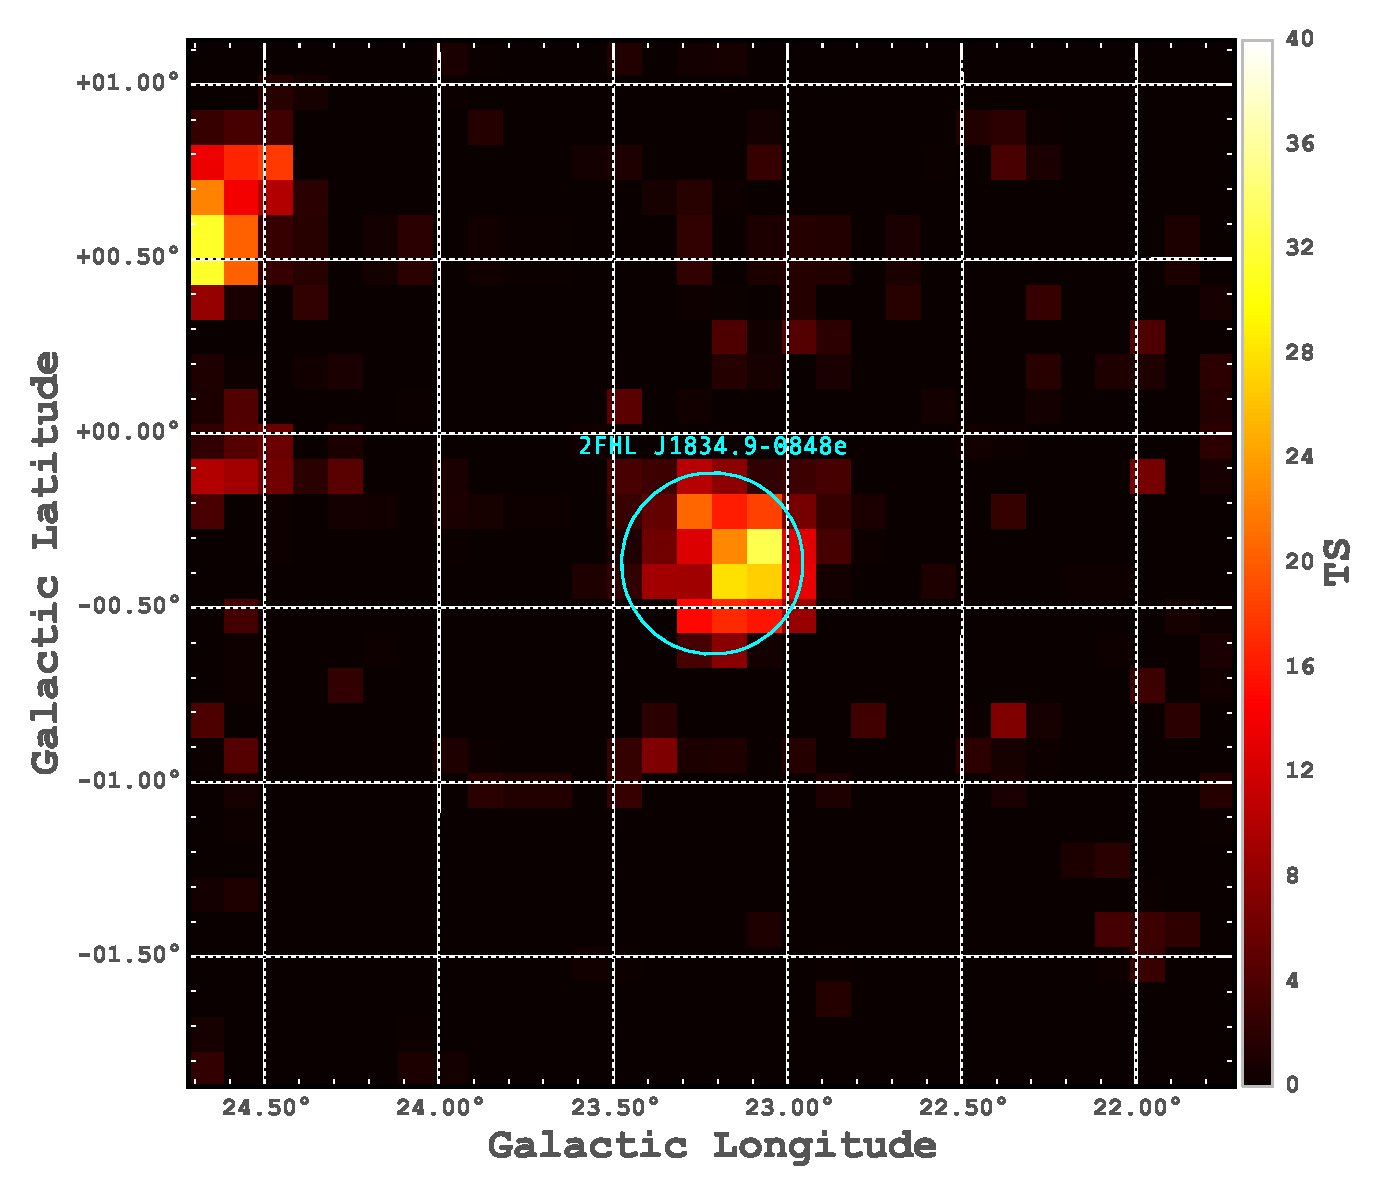
\includegraphics[width=8cm]{Images/l30_b0_ES_2_residTSmap_2FHL_zoom.eps}
		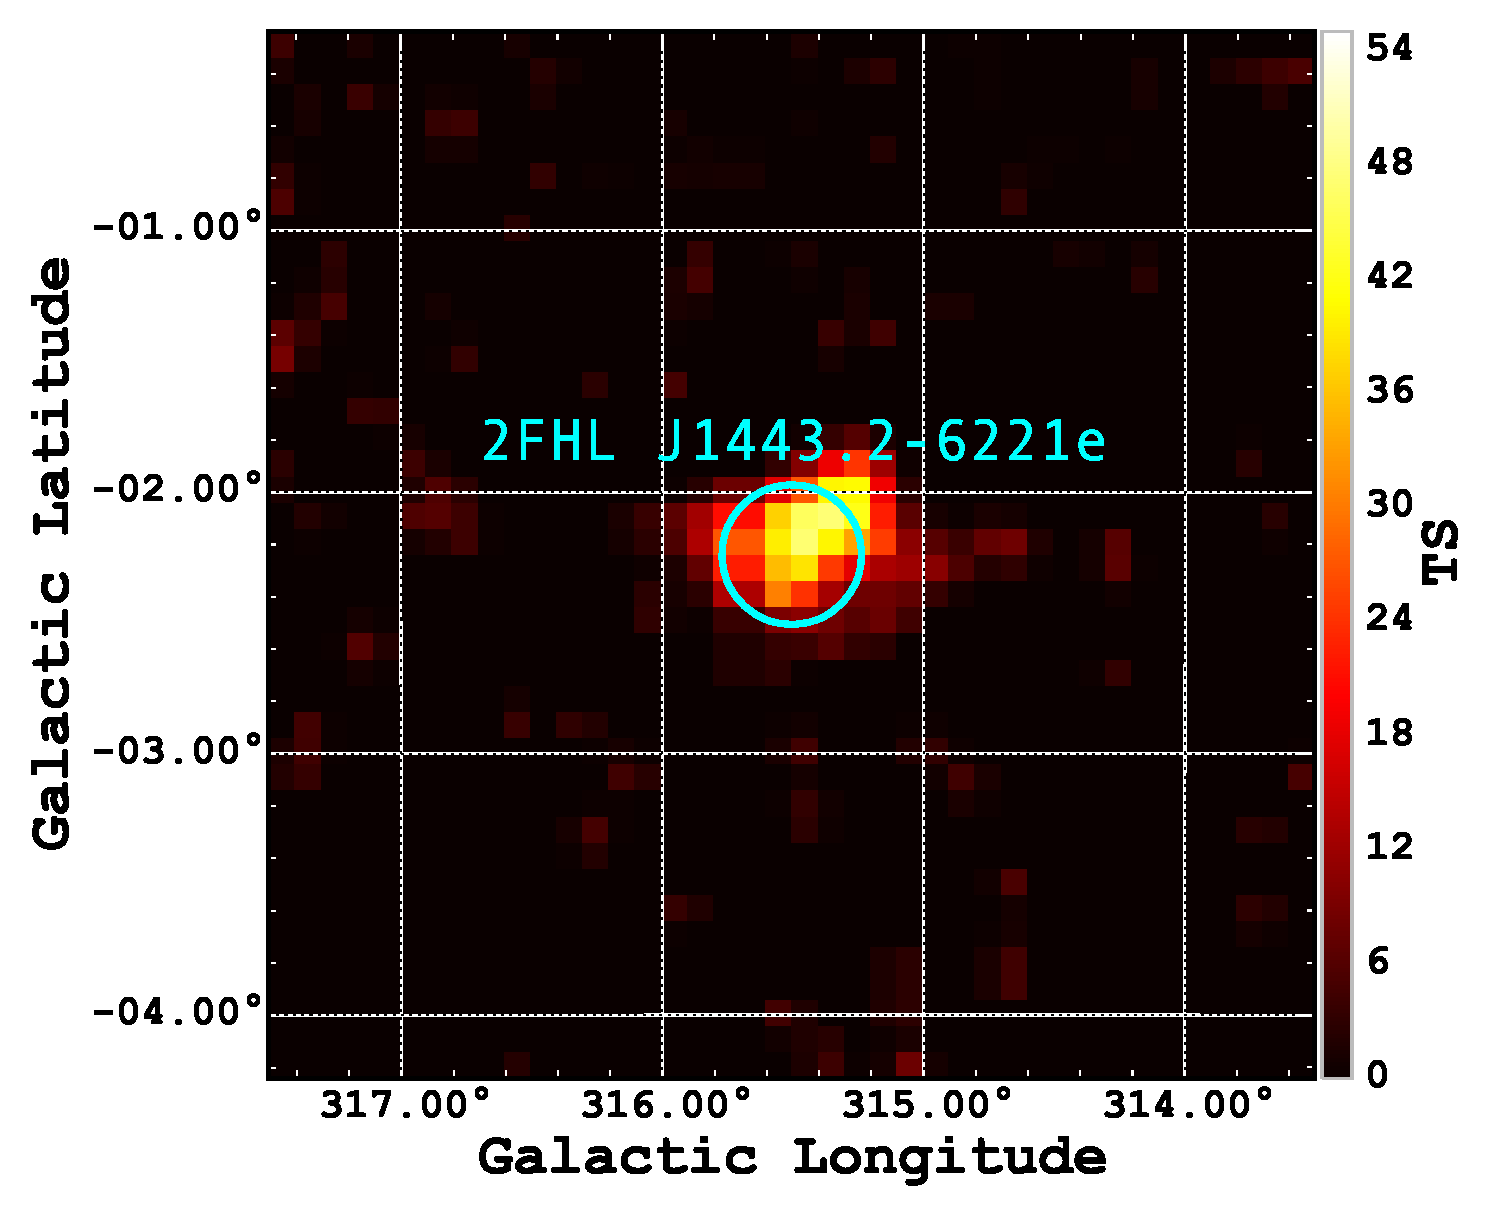
\includegraphics[width=8cm]{Figures/l315_b0_ES_3_residTSmap_2FHL_zoom.eps}
		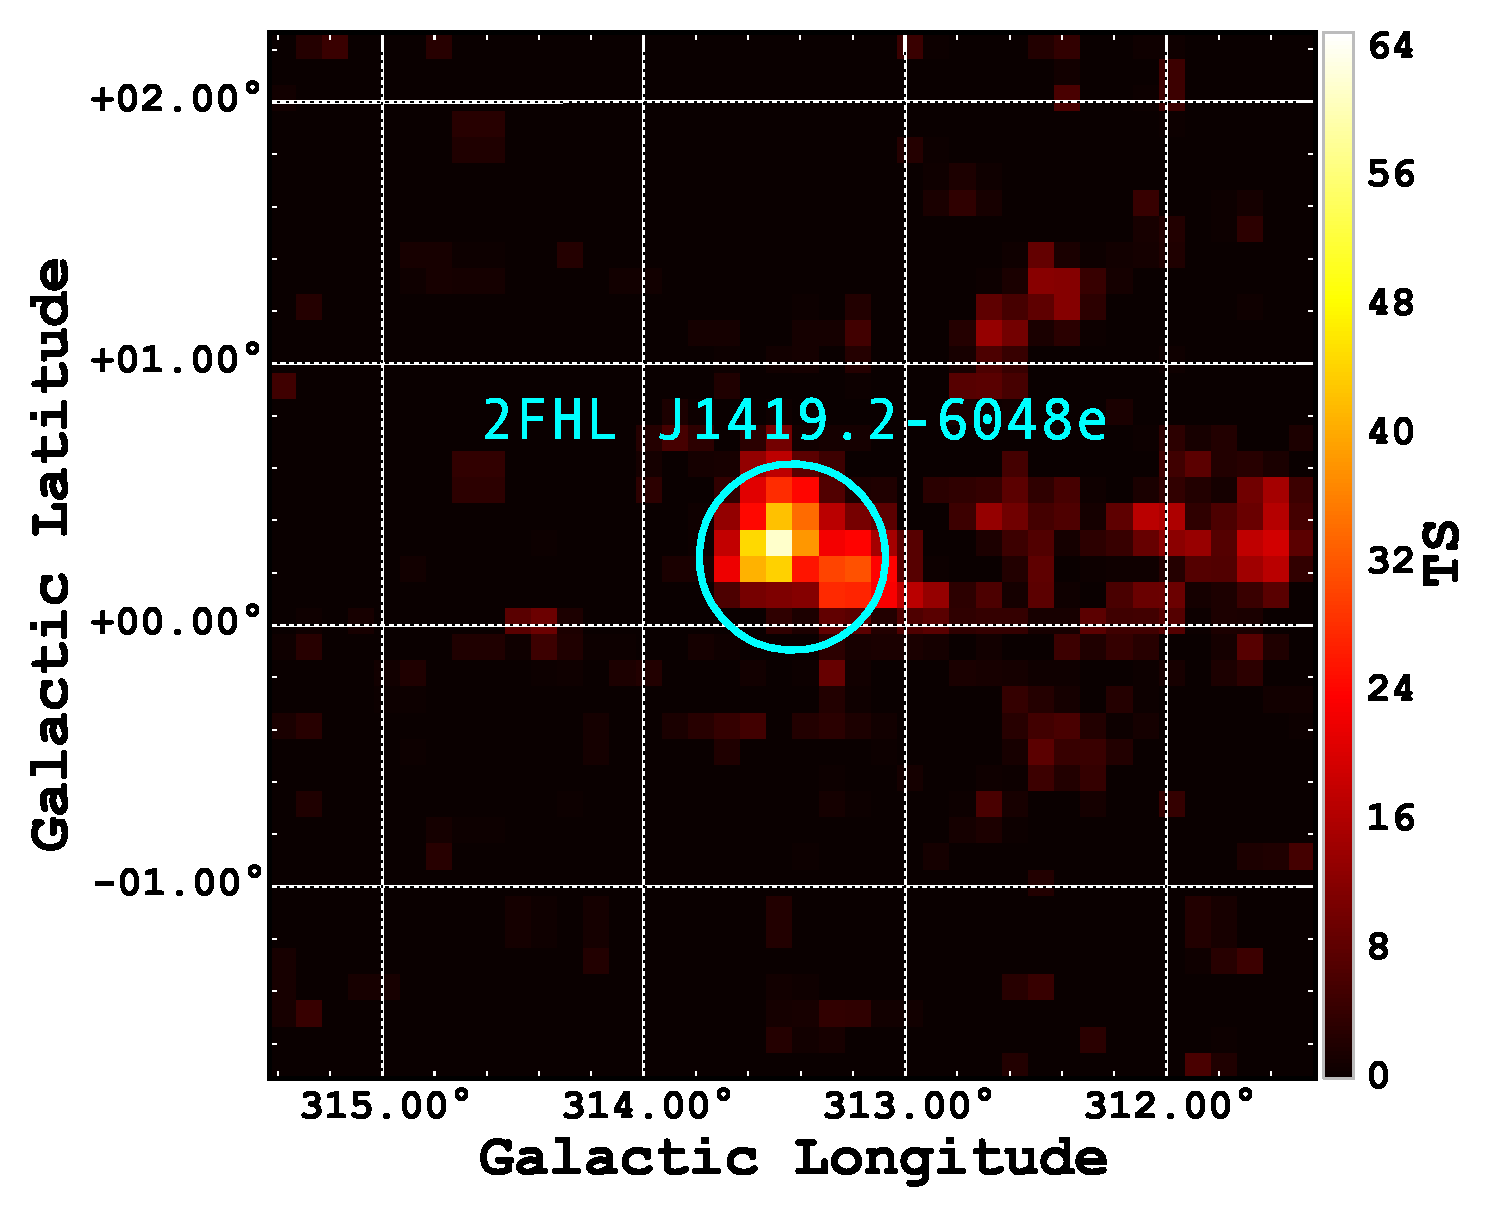
\includegraphics[width=8cm]{Figures/l315_b0_ES_4_residTSmap_2FHL_zoom.eps}
		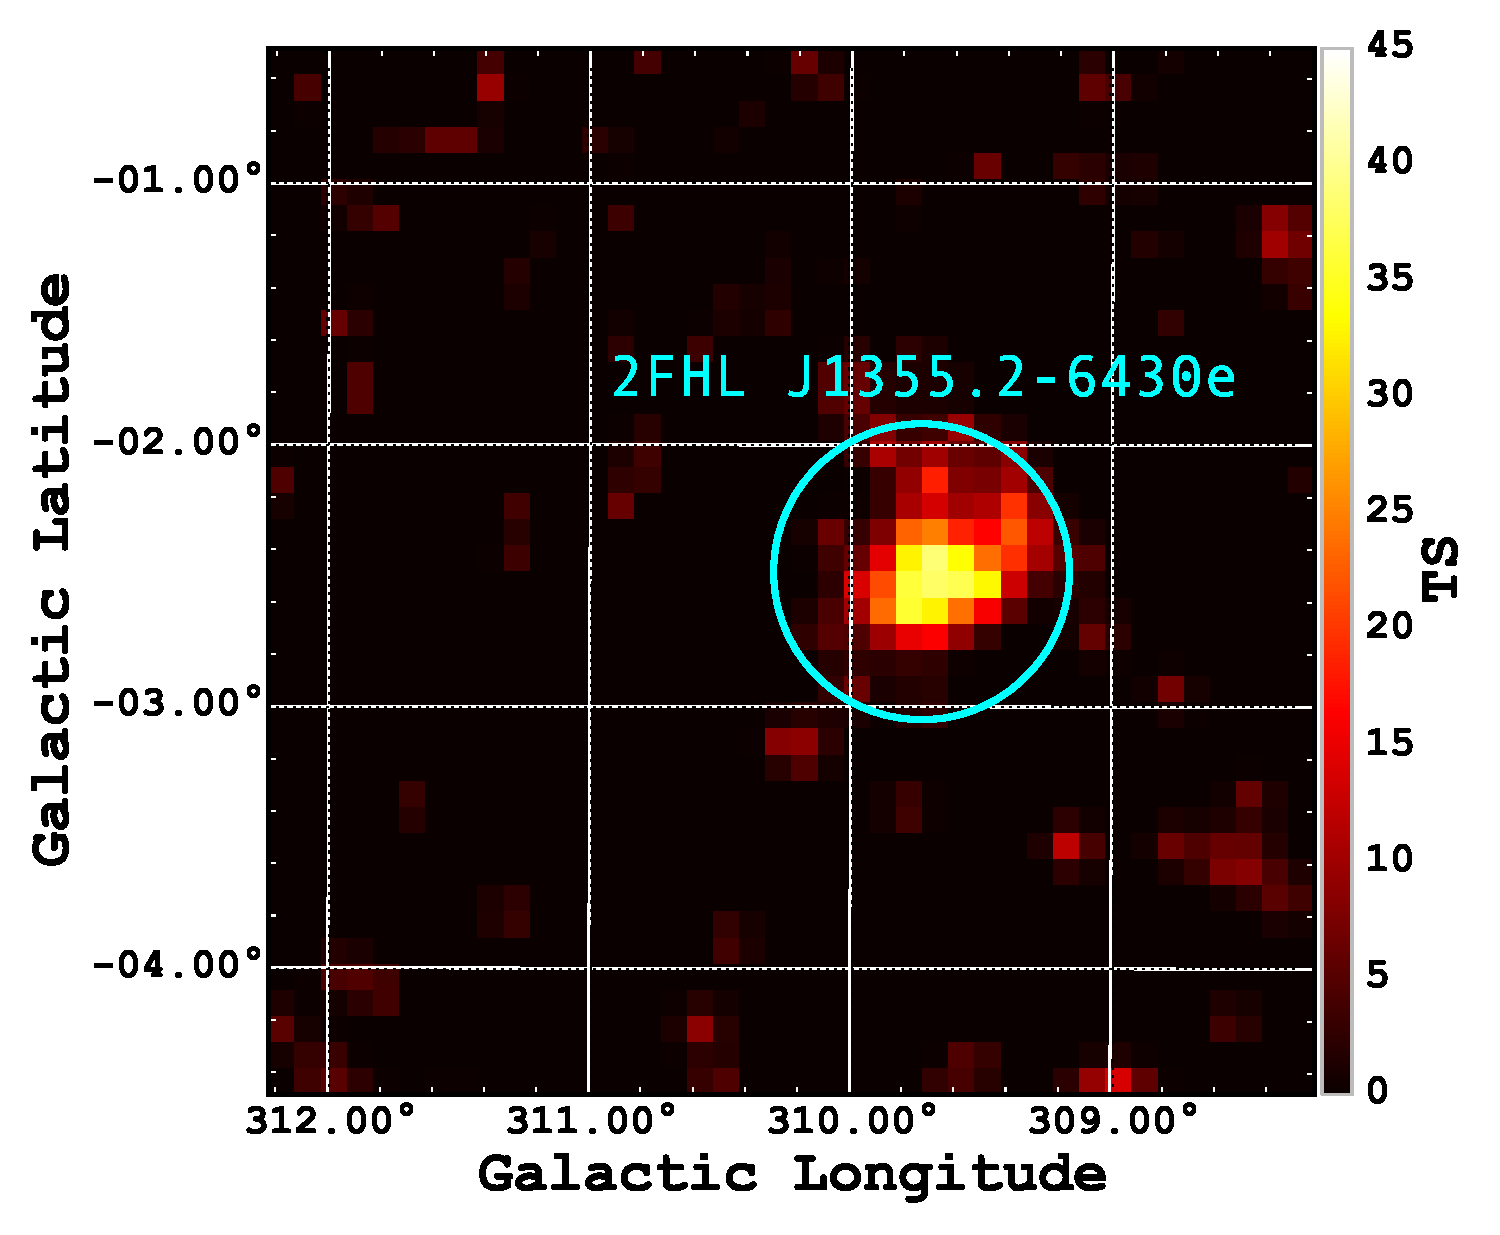
\includegraphics[width=8cm]{Figures/l315_b0_ES_1_residTSmap_2FHL_zoom.eps}
		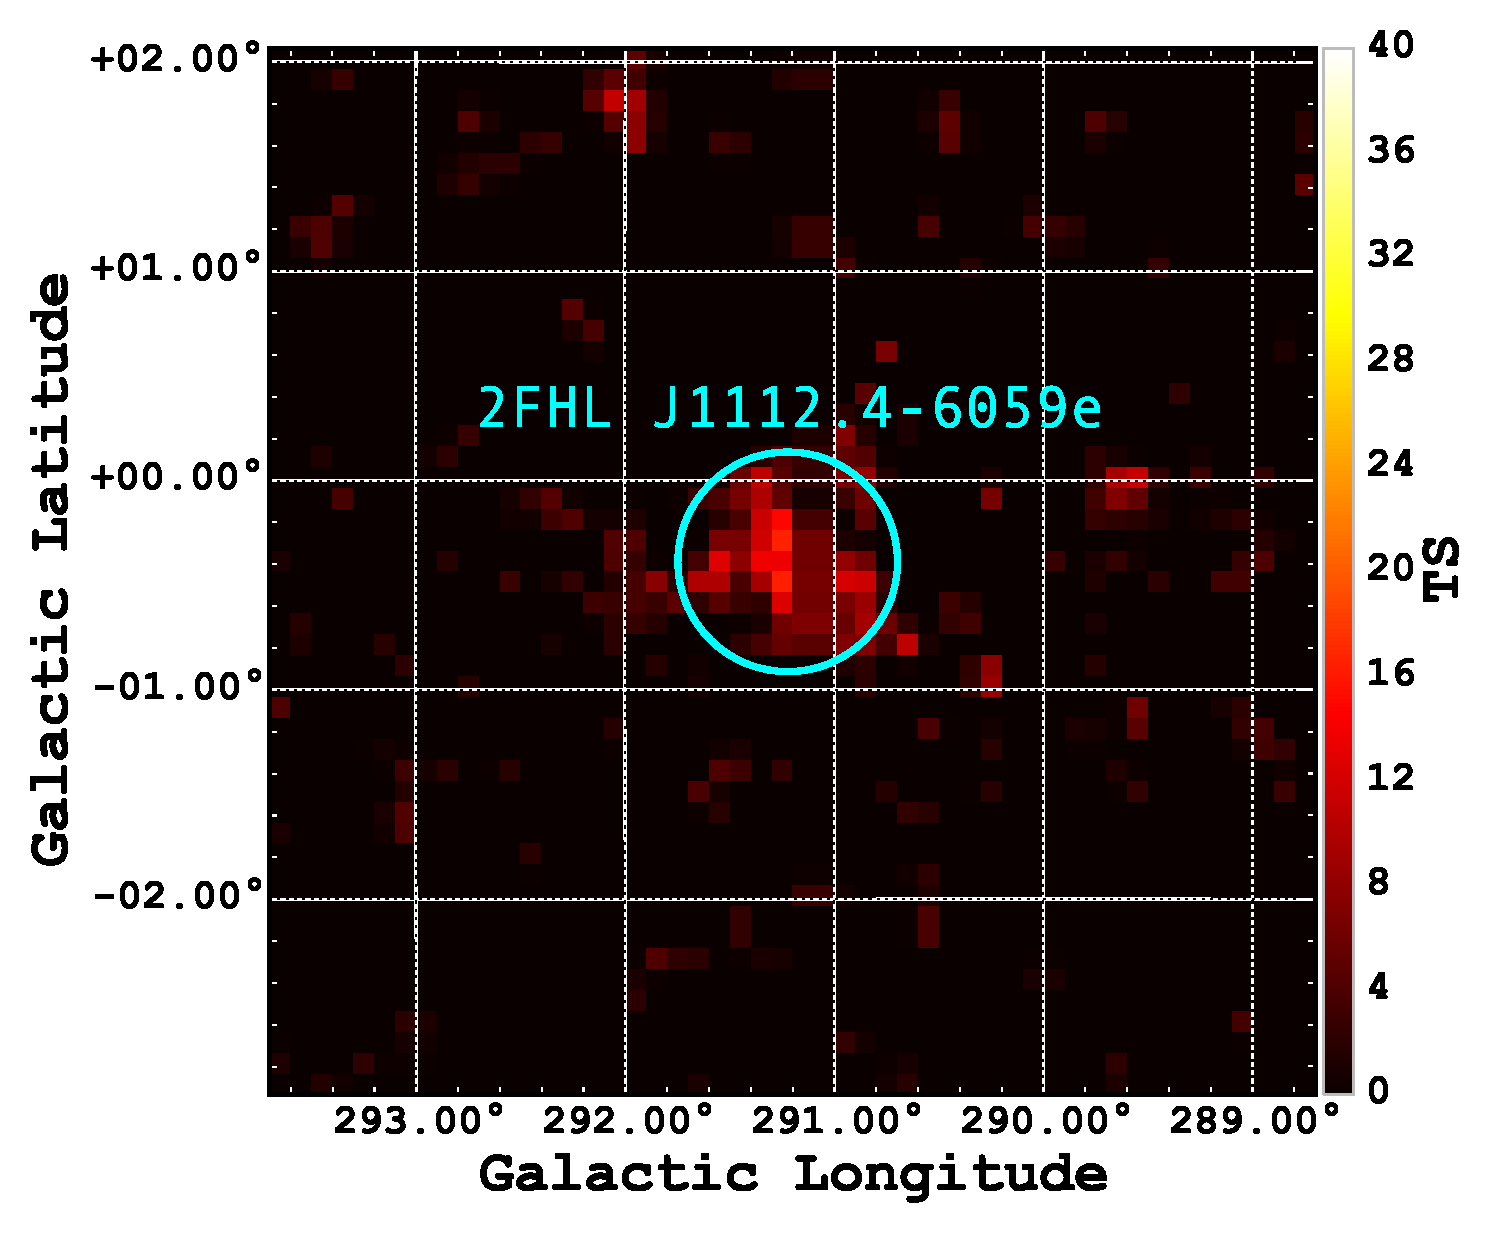
\includegraphics[width=8cm]{Figures/l290_b0_ES_1_residTSmap_2FHL_zoom.eps}
		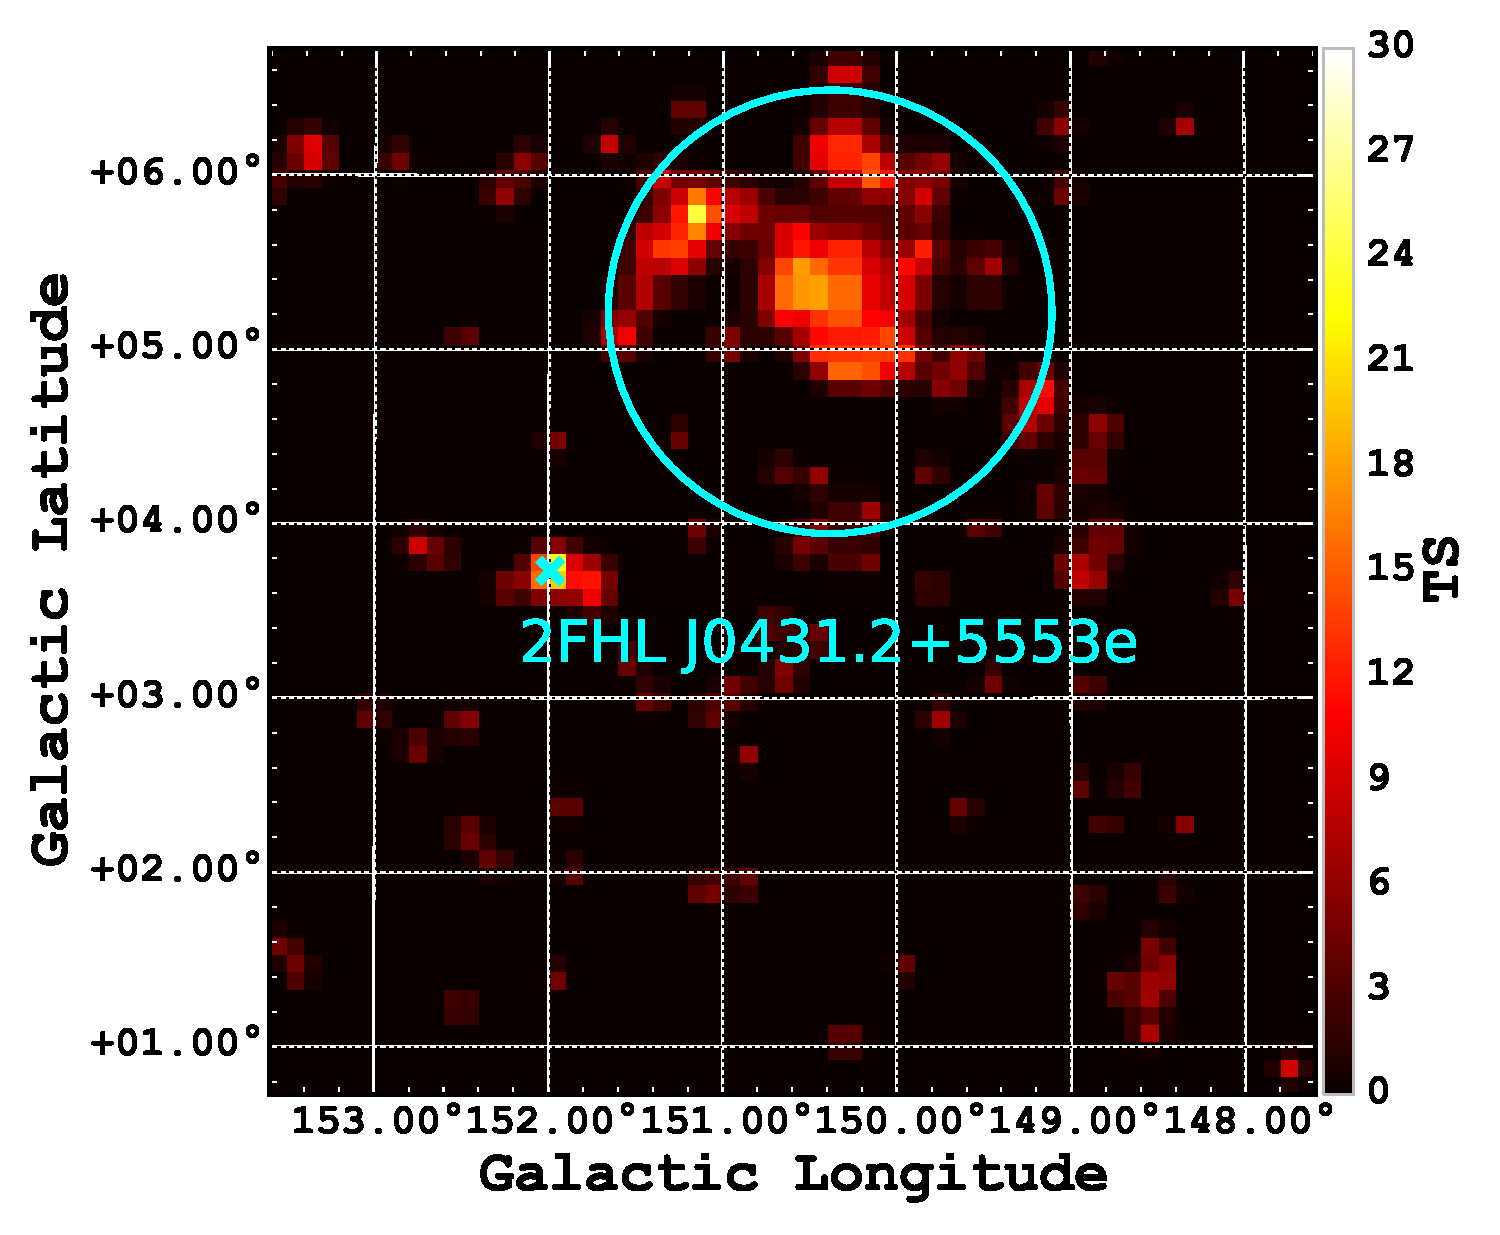
\includegraphics[width=8cm]{Figures/l145_b0_ES_1_residTSmap_2FHL_zoom.eps}
		\caption[TS maps for the five new extended sources.]{TS maps for the five new extended sources described in $\S$ \ref{sec:ESresults}.  Only the Galactic diffuse and isotropic emission are included in the model to highlight the location of emission not associated with the diffuse background. Circles indicate the extents of the fit disks. {The x marker in the bottom panel (2FHL~J0431.2+5553e) shows the location of a point source in the ROI.}
			\label{fig:6ES}}
		
	\end{centering}
\end{figure*}

\section{\label{2FGL:summ}Summary} In this chapter, we have presented the publication on \twofhl, focusing primarily on the Galactic results of the publication and in particular detected extended sources. Extension of addSrcs to search for spatially extended sources, applied to 8 years \jamie{check} of LAT data above 50 \gev. Detected x extended. y were known 3FGL, z were new;y detected as extended at \gev~energies, \Gone ~was brand new. Galactic seem to have harder indices than extra gal, suggests which unid'd in the plane are gal vs. egal. All extended harder than diffuse. Hints of different morphology between \twofhl and \twofgl, didn't study here, but this is one of the motivations for $>$ 10 \gev study.



\begin{deluxetable}{lccclccc}
\setlength{\tabcolsep}{0.04in}
\tablewidth{0pt}
\tabletypesize{\scriptsize}
\tcap{2FHL extended sources previously detected by the {\it Fermi}-LAT \label{tab:extended}}
\tablehead{
\colhead{2FHL Name} & 
\colhead{$l$ [deg]} & 
\colhead{$b$ [deg]} &
\colhead{TS} &
\colhead{Association} &
\colhead{Class} &
\colhead{Spatial model} &
\colhead{Radius [deg]}
}
\startdata
 J0526.6$-$6825e      &    278.843 &    -32.850 & 49.80  & LMC                & gal    & 2D Gaussian 		& 1.87 \\
 J0617.2+2234e        &    189.048 &      3.033 & 398.64 & IC~443             & snr    & 2D Gaussian 		& 0.27 \\
 J0822.6$-$4250e      &    260.317 &	 -3.277 &  63.87 & Puppis A	      & snr    & Disk	     		& 0.37 \\
 J0833.1$-$4511e      &    263.333 &     -3.104 & 49.70  & Vela~X             & pwn    & Disk        		& 0.91 \\
 J0852.8$-$4631e      &    266.491 &     -1.233 & 437.21 & Vela~Jr            & snr    & Disk        		& 1.12 \\
 J1303.4$-$6312e      &    304.235 &     -0.358 & 56.06  & HESS~J1303$-$631   & pwn    & 2D Gaussian 		& 0.24 \\
 J1514.0$-$5915e      &    320.269 &     -1.276 & 165.51 & MSH~15$-$52        & pwn    & Disk        		& 0.25 \\
 J1615.3$-$5146e      &    331.659 &     -0.659 & 128.15 & HESS~J1614$-$518   & spp    & Disk        		& 0.42 \\
 J1616.2$-$5054e      &    332.365 &     -0.131 & 87.18  & HESS~J1616$-$508   & pwn    & Disk        		& 0.32 \\
 J1633.5$-$4746e      &    336.517 &      0.121 & 114.17 & HESS~J1632$-$478   & pwn    & Disk        		& 0.35 \\
 J1713.5$-$3945e      &    347.336 &     -0.473 & 60.98  & RX~J1713.7$-$3946  & snr    & Map         		& 0.56 \\
 J1801.3$-$2326e      &      6.527 &     -0.251 & 50.20  & W~28               & snr    & Disk        		& 0.39 \\
 J1805.6$-$2136e      &      8.606 &     -0.211 & 160.43 & W~30               & snr    & Disk        		& 0.37 \\
 J1824.5$-$1350e      &     17.569 &     -0.452 & 266.09 & HESS~J1825$-$137   & pwn    & 2D Gaussian 		& 0.75 \\
 J1834.9$-$0848e      &     23.216 &     -0.373 &  67.30 & W~41               & spp    & 2D Gaussian		& 0.23 \\
 J1836.5$-$0655e      &     25.081 &      0.136 & 62.72  & HESS~J1837$-$069   & pwn    & Disk        		& 0.33 \\
 J1840.9$-$0532e      &     26.796 &     -0.198 & 163.15 & HESS~J1841$-$055   & pwn    & Elliptical 2D Gaussian & 0.62, 0.38, 39 \\
 J1923.2+1408e        &     49.112 &     -0.466 & 44.60  & W~51C              & snr    & Elliptical Disk        & 0.38, 0.26, 90 \\
 J2021.0+4031e        &     78.241 &      2.197 & 115.97 & Gamma Cygni        & snr    & Disk                   & 0.63 \\
 J2028.6+4110e        &     79.601 &      1.396 & 28.09  & Cygnus Cocoon      & sfr    & 2D Gaussian            & 3.0 \\
\enddata
\tablecomments{~List of the 20 extended sources in 2FHL that were previously detected as extended by the {\it Fermi}-LAT. All these sources are in  3FGL except W41, which is studied by \citet{W41}. The Galactic coordinates $l$ and $b$ are given in degrees. The extension of the disk templates is given by the radius. The extension of the 2D Gaussian templates is given by the $1\sigma$ radius, and the elliptical templates are given by the semi-major axis, semi-minor axis, and position angle (East of North). Association, Class, and Spatial model are as given in \threefgl{}.
}
\end{deluxetable}


\begin{deluxetable}{lcccccccclccc}
\setlength{\tabcolsep}{0.04in}
\tablewidth{0pt}
\tabletypesize{\scriptsize}
\tcap{New 2FHL extended sources 
\label{tab:new_extended}}
\tablehead{
\colhead{2FHL Name} & 
\colhead{$l$ [deg]} & 
\colhead{$b$ [deg]} &
\colhead{TS} & 
\colhead{TS$_{ext}$} &
\colhead{TS$_{2pts}$} &
\colhead{$F_{50}$} & 
\colhead{$\Delta F_{50}$} &
\colhead{$\Gamma$} & 
\colhead{$\Delta \Gamma$} &
\colhead{Association} &
\colhead{Class} &
\colhead{Radius [deg]} 
}
\startdata
 J0431.2+5553e        &    150.384 &      5.216 &  87.9 & 83.4  & 26.2    &  11.70 &       2.11 &    1.66 &         0.20 & G~150.3+4.5     & snr     & 1.27 $\pm$  0.04 \\
 J1112.4$-$6059e      &    291.222 &     -0.388 &  80.9 & 68.3   & 22.5    &  12.80 &       2.36 &    2.15 &         0.28 & PSR~J1112$-$6103  & pwn     & 0.53 $\pm$ 0.03 \\
 J1355.2$-$6430e      &    309.730 &     -2.484 &  82.3 & 31.8   & 12.9     &  9.59  &       1.95 &    1.56 &         0.22 & PSR~J1357$-$6429  & pwn     & 0.57 $\pm$ 0.02 \\
 %J1407.3$-$6116e      &    311.924 &      0.259 &  68.66 & 30.00       &  14.70 &       2.63 &    2.58 &         0.28 & \nodata         & \nodata & 0.38 \\
 J1419.2$-$6048e      &    313.432 &      0.260 & 109.3 & 49.1   & 15.6    &  17.60 &       2.80 &    1.87 &         0.19 & PSR~J1420$-$6048  & pwn     & 0.36 $\pm$ 0.03  \\
 J1443.2$-$6221e      &    315.505 &     -2.239 &  75.6 & 29.9   & 19.2   &  7.23  &       1.70 &    2.07 &         0.30 & SNR~G315.4$-$2.3  & snr     & 0.27 $\pm$  0.03 \\
\enddata
\tablecomments{~List of the 5 new extended sources in 2FHL. All sources are characterized by a uniform disk template whose radius and uncertainty therein is given in the last column. $l$ and $b$ are Galactic coordinates. All coordinates are shown in degrees. TS is the test statistic. ${\rm TS_{ext}} $ is the signicance of extension (\ref{2fhl:newES}). TS$_{2pts}$ is the TS of two simultaneously fit point sources  (\ref{2fhl:newES}). $F_{50}$ and $\Delta F_{50}$ are the integrated photon flux between 50~GeV and 2~TeV and its uncertainty in units of $10^{-11}$~photon~cm$^{-2}$~s$^{-1}$. $\Gamma$ and $\Delta \Gamma$ are the photon  index and its uncertainty from a power-law fit. Association lists the primary overlapping source and Class the suspected source type.  All uncertainties are $1\sigma$ uncertainties.}
\end{deluxetable}

\section{Scratch}
Add stuff to first section about extension fitting with pointlike
In addition to being optimized for speed and large-scale studies (\ie{} those including many sources), \ptlike{}

I should probably give more detail about Josh's code than I did for just the regular pointlike?

Next, get into Josh's extension additions to pointlike
It accomplishes this by binning the sky in  

Should I say some things about why extension fitting is important in general?
